% Robotics Institute Technical Report
%
% Unofficial Template for RI Technical Reports
% Use with latex2e
%
% Modified by: David Fouhey, Oct 2014
% Created by: Daniel Morris, Dec 2000
%
% DM:
%   Since I was unable to find a template for Technical Reports, I made up my
%   own.  Use it at your own risk -- as I am not a latex guru.


\documentclass[twoside,10pt]{report}
\usepackage{marginnote}
\usepackage[left=1.5in,right=1.5in,top=1.5in,bottom=1.5in]{geometry}
\usepackage[usenames,dvipsnames]{xcolor}
\usepackage{graphicx,amsmath,amssymb,multirow,booktabs,color,verbatim,cite,url,placeins}
\usepackage{layouts,array,wrapfig}
\usepackage[normalem]{ulem}
\usepackage{tgpagella}

\usepackage{array}
\newcolumntype{P}[1]{>{\centering\arraybackslash}p{#1}}

%%%%%%%%%%%%%%%%%%%%%%%%%%%%%%%%%%%%
%DF: Nuke all the notes by using 
%the second note definition below
\newcommand{\note}[1]{\textcolor{red}{#1}}
%\newcommand{\note}[1]{}


%I usually like to put more figures on a page with text than latex's
%default
\renewcommand{\textfraction}{0.05}
\renewcommand{\topfraction}{0.9}
\renewcommand{\floatpagefraction}{0.8}

\newcommand{\clearemptydoublepage}{\newpage{\pagestyle{empty}\cleardoublepage}}

%Table of contents stuff
\setcounter{tocdepth}{1}

\newcommand\MyBox[2]{
  \fbox{\lower0.75cm
    \vbox to 1.5cm{\vfil
      \hbox to 1.5cm{\hfil\parbox{1.2cm}{#1\\#2}\hfil}
      \vfil}%
  }%
}

\begin{document}

\title{2 Legit 2 Quit}
\author{JJ Gibson}


%title page
\thispagestyle{empty}
%Put the date below the TR number
\date{}

\begin{center}

%{\Huge \bf Future Near-Collision Prediction \\ \vspace{0.5cm} from Monocular Video} \\
{\Huge \bf Real-Time Collision Forecasting \\ \vspace{0.5cm} from Monocular Video} \\
\vspace{1cm}  
{\Large Aashi Manglik} \\
\vspace{1cm} 

%%%%%%%%%%%%%%%%%%%%%%%%%%%%%%%%%
%Include in final thesis
%\vspace{-0.5cm}
%{\large CMU-RI-TR-00-00}
%\vspace{2cm}
%%%%%%%%%%%%%%%%%%%%%%%%%%%%%%%%%

{\Large June 3, 2019} \\
\vspace{2cm}
{\Large
The Robotics Institute\\
Carnegie Mellon University\\
Pittsburgh, Pennsylvania 15213\\
}
\vspace{1cm}
{\Large
{\bf Thesis Committee:}\\
Prof. Kris M. Kitani, Chair, CMU \\
Prof. Aaron Steinfeld, CMU \\
Ishani Chatterjee, CMU \\
}
\vspace{2cm}
\par ~ \\
{\large \it Thesis proposal submitted in partial fulfillment of the \\
    requirements for the degree of Master of Science in Robotics}
\vfill
{\large \copyright Aashi Manglik, 2019}
\end{center}



\clearpage


%start the forematter 
\pagenumbering{Roman}
\clearemptydoublepage
\setcounter{page}{1}

\begin{centering} \section*{Abstract} \end{centering}
We explore the possibility of using a single monocular camera to forecast the time to collision between a suitcase-shaped robot being pushed by its user and other nearby pedestrians. We develop a purely image-based deep learning approach that directly estimates the time to collision without the need of relying on explicit geometric depth estimates or velocity information to predict future collisions. While previous work has focused on detecting immediate collision in the context of navigating Unmanned Aerial Vehicles, the detection was limited to a binary variable (\emph{i.e.}, collision or no collision). We propose a more fine-grained approach to collision forecasting by predicting the exact time to collision in terms of milliseconds, which is more helpful for collision avoidance in the context of dynamic path planning. To evaluate our method, we have collected a novel large-scale dataset of over 13,000 indoor video segments each showing a trajectory of at least one person ending in a close proximity (a near collision) with the camera mounted on a mobile suitcase-shaped platform. Using this dataset, we do extensive experimentation on different temporal windows as input using an exhaustive list of state-of-the-art convolutional neural networks (CNNs). Our results show that our proposed multi-stream CNN is the best model for predicting time to near-collision. The average prediction error of our time to near collision is $0.75$ seconds across our test environments.


\tableofcontents
\clearpage

%%%%%%%%%%%%%%%%%%%%%%%%%%%%%%%%%
%Include in final thesis
%\clearpage \listoffigures
%\clearpage \listoftables
%\clearpage
%%%%%%%%%%%%%%%%%%%%%%%%%%%%%%%%%

%start the actual document
\pagenumbering{arabic}
\setcounter{page}{1}


\chapter{Introduction}
\label{chap:introduction}
%Man, robots are hard.... But the only book you'll need is
%\cite{Gibson79}. \note{Is self-citing tacky?}

%%%%%%%%%%% First paragraph - Motivating time to collision %%%%%%%%%%%%%
Automated collision avoidance technology is an indispensable part of mobile robots. As an alternative to traditional approaches using multi-modal sensors, purely image based collision avoidance strategies \cite{gandhi}, \cite{DroNet} have recently gained attention in robotics. These image-based approaches use the power of large data to detect immediate collision as a binary variable - collision or no collision. In this work, we propose a more fine-grained approach to predict the exact time to near-collision from images, with a much longer prediction horizon.  

   \begin{figure}[t]
      \centering
      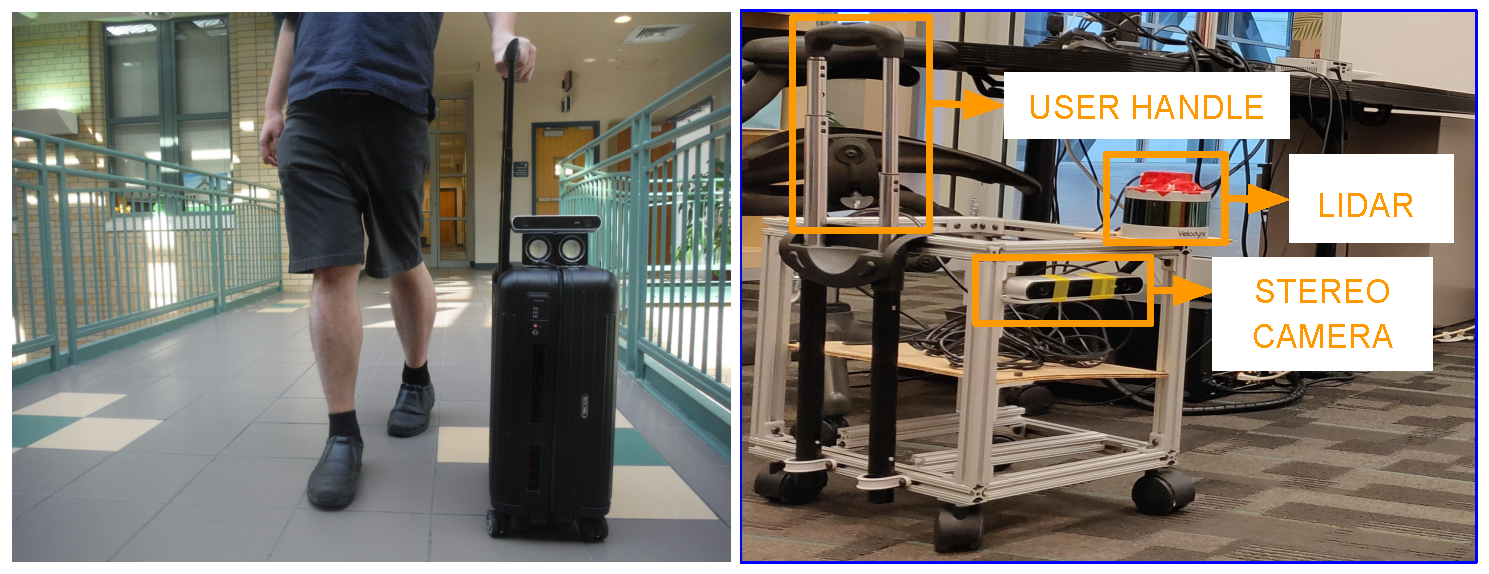
\includegraphics[height=5.5cm, width=\columnwidth]{figs/aspect_ratio_setup.pdf}
      \caption{The left image shows an assistive suitcase with a camera sensor and speaker to guide people. The right image shows the corresponding suitcase-shaped training prototype mounted with stereo camera and LIDAR for data collection.}
      \label{fig:setup}
   \end{figure}

%%%%%%%%%% Second paragraph - Anticipating common arguments %%%%%%%%%%%%%%%%%%%
A method frequently used for forecasting time to near-collision is to track the 3D location of the surrounding pedestrians and extrapolate their trajectories using a constant velocity model \cite{SIPP}, \cite{BBeep}. When it is possible to use high quality depth imaging devices, this type of physics-based modeling can be very accurate. However, physics-based approach can also be prone to failure in the presence of sensor noise and uncertainty in detection of nearby pedestrians. Small mistakes in the estimation of depth (common to low-cost depth sensors) or noise in 2D bounding box detection (common to image-based object detection algorithms) can be misinterpreted to be very large changes of velocity. Many physics-based approaches can be brittle in the presence of such noise. Accordingly, errors in either pedestrian detection, tracking or data association can result in very bad future trajectory estimates. Other more advanced physics-based models and decision-theoretic models also depend heavily on accurate state estimates of nearby people and can be significantly influenced by sensor and perception algorithm noise. We propose to address the issue of sensor noise and perception algorithm noise by directly estimating the time to near-collision from a sequence of images.
   
%%%%%%%%% Fourth paragraph - How did we go about creating the dataset? %%%%%%%%%%%%%%%%%%%%%%%%   
To create a dataset for learning time to collision, we designed a training prototype as shown in Fig. \ref{fig:setup}. It is both unnatural and infeasible to record or insist that people actually collide with the mobile platform to collect large scale data. As an abstraction, we define the presence of a person within a 1 meter radius around the mobile platform as a near-collision. If a person other than the user is present within this radius, we mark it as a near-collision that should be forecasted using an earlier segment of video. The proposed approach is designed for a mobile robot that is being pushed by a person with visual impairment as shown in Fig. \ref{fig:setup}. The goal of the system is to forecast the time to near collision, at most 6 seconds before the near collision event. While most of the existing datasets for human trajectory prediction are from a fixed overhead camera \cite{2009YoullNW}, \cite{UCY}, our dataset of \textbf{13,658} video segments targets the first-person view which is more intuitive for mobile robots. In the work on robust multi-person tracking from mobile platforms \cite{Andreas}, the dataset is egocentric at walking speed but with 4788 images it is insufficient to deploy the success of convolutional neural networks. 


%%%%%%%%% Fifth paragraph - Technical part, how exactly we are learning %%%%%%%%%%%%%%%
We formulate the forecasting of time to near-collision as a regression task. To learn the mapping from spatial-temporal motion of the nearby pedestrians to time to near-collision, we learn a deep network which, takes a sequence of consecutive frames as input and outputs the time to near-collision. To this end, we evaluate and compare two popular video network architectures in the literature: (1) The high performance of the image-based network architectures makes it appealing to reuse them with as minimal modification as possible. Thus, we extract the features independently from each frame using an image-based network architecture (\emph{e.g.}, VGG-16) and then aggregate the features across the temporal channels; (2) It is also natural to directly use a 3D ConvNet (\emph{e.g.}, I3D \cite{i3d}) to learn the seamless spatial-temporal features.

Moreover, it is a nontrivial task to decide how many past frames should form the input. Thus, we do extensive experimentation on different temporal windows as input using aforementioned video network architectures. Our results show that our proposed multi-stream CNN trained on the collected dataset is the best model for predicting time to near-collision.


In summary, the contributions of our work are as follows: (1) We contribute a large-scale dataset of \textbf{13,658} egocentric video snippets of humans navigating in indoor hallways. In order to obtain ground truth annotations of human pose, the videos are provided with the corresponding 3D point cloud from LIDAR; (2) We explore the possibility of forecasting the time to near-collision directly from a single RGB camera; (3) We provide an extensive analysis on how current state-of-the-art video architectures perform on the task of predicting time to near-collision on the proposed dataset and how their performance varies with different temporal windows as input.

\clearpage

\chapter{Related Work}
\label{chap:related_work}
\noindent
\section{Monocular-Based Collision Avoidance} 

Existing monocular collision avoidance systems mostly focus on avoiding the immediate collision at the current time instant. Learning to fly by crashing \cite{gandhi} presented the idea of supervised learning to navigate an unmanned aerial vehicle (UAV) in indoor environments. The authors create a large dataset of UAV crashes and train an AlexNet \cite{alexnet} with single image as input to predict from one of these three collision avoidance actions - go straight, turn left or turn right. Similarly, DroNet \cite{DroNet} trains a ResNet-8 \cite{resnet} to safely navigate a UAV through the streets of the city.
% in contrast to traditional map-localize-plan approach. 
DroNet takes the images from an on-board monocular camera on UAV and outputs a steering angle along with the collision probability. 

While predicting an action to avoid the immediate collision is useful, it is more desirable to predict a possible collision in the short future.

Therefore, our work focuses on forecasting the exact time to a possible collision occurring within next 6 seconds, which will be helpful for collision avoidance in the context of dynamic path planning \cite{SIPP}, \cite{time-bounded}, \cite{vemula2016path}. For planning in the presence of dynamic obstacles such as pedestrians, Safe Interval Path Planning (SIPP) \cite{SIPP} defines a safe interval as a contiguous period of time during which there is no collision. While the number of timesteps may be unbounded, the number of safe intervals is finite making the search space tractable for the planner. Our approach finds the time-to-collision in real-time and thus can be useful for SIPP planner to define safe interval. Another path planning algorithm called time-bounded lattice \cite{time-bounded} merges together short-term planning in time with less expensive long-term planning without time. This planner computes a single bound for how long the planning should be done in time. The near-collision time predicted by our approach can thus serve the purpose of deciding the time bound for the short-term spatio-temporal planning.    

\noindent\\
\section{Predicting Time to Collision by Human Trajectory}

Instead of predicting the time to collision directly from images, one can also predict the human trajectories \cite{socialGAN}, \cite{socialLSTM}, \cite{anirudh}, \cite{2009YoullNW}, \cite{ziebart2009planning} as the first step, then the time to collision can easily be computed from the predicted trajectories.
% \textcolor{red}{need brief explanation for each paper here.}
\cite{2009YoullNW} introduces a dynamic model for human trajectory prediction in a crowd scene by modeling not only the history trajectory but also the surrounding environment. \cite{socialLSTM} proposes a LSTM model to learn general human movement pattern and thus can predict the future trajectory. As there are many plausible ways that humans can move, \cite{socialGAN} proposes to predict diverse future trajectories instead of a deterministic one. \cite{anirudh} proposes an attention model, which captures the relative importance of each surrounding pedestrian when navigating in the crowd, irrespective of their proximity.


However, in order to predict future trajectory reliably, these methods rely on accurate human trajectory history. This usually involves multi-people detection and tracking, and thus has two major disadvantages: (1) Data association is very challenging in crowded scenarios. Small mistakes can be misinterpreted to be very large changes of velocity, resulting in very bad trajectory estimate; (2) Robust multi-person tracking from mobile platform is often time-consuming. For example, \cite{Andreas} takes 300ms to process one frame on a mobile GPU, making it impossible to achieve real-time collision forecasting. 

In contrast, our approach can predict the time to collision directly from a sequence of images, without requiring to track the surrounding pedestrians explicitly. We demonstrate that our data-driven approach can implicitly learn reliable human motion and also achieve real-time time to collision.


\noindent\\
\section{Learning Spatio-Temporal Feature Representation}

Existing video architectures for spatio-temporal feature learning can be split into two major categories. To leverage the significant success from image-based backbone architectures (\emph{e.g.}, VGG and ResNet) pre-trained on large-scale image datasets such as ImageNet \cite{imagenet} and PASCAL VOC \cite{pascalVOC}, methods in the first category reuse the 2D ConvNet to extract features from a sequence of images with as minimal modifications as possible. For example, \cite{BeyondSS} proposes to extract the image-based features independently from each frame using GoogLeNet and then apply a LSTM \cite{lstm} on the top for feature aggregation for video action recognition.

The second category methods explore the use of 3D ConvNets for video tasks \cite{C3D}, \cite{videoResNet}, \cite{p3d}, \cite{two-stream} that directly operate 3D spatio-temporal kernels on video inputs. While it is natural to use 3D ConvNets for spatio-temporal feature learning, 3D ConvNets are unable to leverage the benefits of ImageNet pretraining directly and often have huge number of parameters which makes it most likely to overfit on small datasets. Recently, the two-stream inflated 3D ConvNet (I3D) \cite{i3d} is proposed to mitigate these disadvantages by inflating the ImageNet-pretrained 2D weights to 3D. Also, the proposed large-scale video dataset, Kinetics, has shown to be very successful for 3D kernel pre-training.
 

To validate how current state-of-the-art video architectures perform on the task of predicting time to near-collision on the proposed dataset, we evaluate methods from both categories in our experiments.





\clearpage

\chapter{Dataset}
\label{chap:dataset}
% \begin{figure}
%     \centering
%     \includegraphics[scale=0.40]{figs/setup.jpg}
%     \caption{Suitcase-shaped mobile system with stereo camera and LIDAR}
%     \label{fig:setup}
% \end{figure}

%%%%%%%%% Feb 18 %%%%%%%%%

\begin{table*}[ht]
\centering
\caption {Video Datasets with egocentric viewpoint} \label{tab:data} 
\begin{tabular}{|P{0.25\textwidth}|P{0.25\textwidth}|P{0.25\textwidth}|P{0.25\textwidth}|} \hline
Dataset & Number of near-collision video sequences & Structure of scenes & Setup for recording \\ \hline 
\textbf{Ours} (Near-collision)  & 13,685 & Indoor hallways & Suitcase  \\ \hline 
UAV crashing \cite{gandhi} & 11,500 & Indoor hallways & UAV  \\ \hline  
DroNet \cite{DroNet} & 137 & Inner-city & Bicycle  \\ \hline 
%Collision trajectory \cite{ziebart} & 166 & Kitchen Area & Laser range finders & Fixed \\ \hline  
Robust Multi-Person Tracking \cite{Andreas} & 350  & Busy inner-city & Chariot \\ \hline   
\end{tabular}
\end{table*}

We sought to analyze a large-scale, real-world video dataset in order to understand challenges in prediction of near-collision events. However, based on our survey, existing datasets had a small number of interaction events as reported in Table \ref{tab:data} and lacked diversity in the capture settings. Therefore, in order to train robust CNN models that can generalize across scenes, ego-motion, and pedestrian dynamics, we collected an extensive dataset from a mobile perspective. Next, we describe our hardware setup and methodology for data collection. 
%We further provide the algorithm used for automatic ground truth annotation. 

\section{Hardware Setup}
The mobile platform used for data collection is shown in Fig.~\ref{fig:setup}, and includes a stereo camera and LIDAR sensor. While during inference we only utilize a monocular video, the stereo camera serves two purposes. First, it provides a depth map to help in automatic ground truth annotation. Second, it doubles the amount of training data by providing both a left and right image perspective which can be used as separate training samples. However, during the process of automatic data annotation, it was observed that the depth maps from stereo camera are insufficient for extracting accurate distance measurements. In particular, when the pedestrian is close to camera the depth values are missing at corresponding pixels due to motion blur. To resolve this issue we utilize a LIDAR sensor, which is accurate to within a few centimeters. The images and corresponding 3D point clouds are recorded at the rate of 10Hz.     

% The mobile platform shown in \ref{fig:setup} is used to collect videos inside university buildings. The data is split into train and test as follows:
% \begin{itemize}
% \item Training images - 10685 (2106 positive and 8579 negative)  
% \item Test images - 3563 (687 positive and 2876 negative)
% \end{itemize}
%  The camera and LIDAR are calibrated using \cite{calibration}. We used Faster RCNN object detector to detect the pedestrian in RGB image and recorded the ground truth position in world from projected point cloud. 

\section{Camera-LIDAR Extrinsic Calibration}
We use the camera and the LIDAR for automatic ground truth label generation. The two sensors can be initially calibrated with correspondences~\cite{Autoware,calibration}. An accurate calibration is key to obtaining the 3D position of surrounding pedestrians and annotating the large number of videos in our dataset. Let $R$ and $t$ denote the rotation matrix and the translation vector defining the rigid transformation between the LIDAR to the camera frame and $K$ the $3 \times 3$ intrinsic matrix of camera. Then, the LIDAR 3D coordinates $(x, y, z)$ can be related to a pixel in the image with coordinates $(U,V) = (\frac{u}{w}, \frac{v}{w})$ using following transformation:
%U = \frac{u}{w}; V = \frac{v}{w}
\begin{equation}\label{eq:Rt}
    \begin{bmatrix}u \\ v \\ w\end{bmatrix} = K[R \mid -R^{T}t] \begin{bmatrix} x \\ y \\ z \\ 1\end{bmatrix}
\end{equation}

Given this calibration, we can now project LIDAR points onto the image and obtain estimated depth values for the image-based pedestrian detection. 

%$$
%$$
%Here, . 
%% An example of projection of point cloud onto the image is shown in figure \ref{fig:projection}.
%% Show the pipeline - image showing projected point cloud, heatmap from GRADCAM 
%% Number of training and test images 

% \begin{figure}[h]
%     \centering
%     \includegraphics[scale=0.35]{figs/point_cloud_projected_over_image.eps}
%     \caption{Point cloud projected on image to extract 3D pose}
%     \label{fig:projection}
% \end{figure}


%For people detection, we employ a state-of-the-art person detection (Faster-R-CNN \cite{fasterRCNN}). Given a person detection, we can then compute its 3D location in the scene from the corresponding 3D point cloud.

%However, Autoware requires 30-40 poses of calibration target to output accurate transformation and thus we later shifted to \cite{calibration} which only requires 1-3 poses.  

\section{Large-Scale Data Collection and Annotation}
The platform is pushed through three different university buildings with low-medium density crowd. Our recorded videos comprise of cafeteria and hallways of varying styles. 
%Each image is automatically annotated with a binary label using algorithm \ref{algo}. 
%An illustration of the resulting processing is shown in Fig. \ref{fig:gt}. A positive binary label indicates the presence of humans within the radius of 1 meter around the setup. As presented in line 3 of algorithm \ref{algo}, we detect the persons' bounding boxes by applying Faster RCNN \cite{fasterRCNN} on image and thus the persons behind the setup are not considered. 
We experimented with several techniques for obtaining pedestrian detections in the scene from the image and LIDAR data. As 2D person detection is a well-studied problem, we found an image-based state-of-the-art person detection (Faster-R-CNN \cite{fasterRCNN}) to perform well in most cases, and manually inspect and complete any missing detections or false positives. To obtain the 3D position of each detected bounding box, we compute a median distance of its pixels using the 3D point cloud. An illustration of the resulting processing is shown in Fig. \ref{fig:gt}. Each image is annotated with a binary label where a positive label indicates the presence of at least one person within a meter distance from setup. We understand that the people in camera's view who move in the same direction as camera might not be important for collision. However, the number of such instances is insignificant in our dataset. \\
%Some of the halls also have students sitting on study tables who are also referred to as pedestrians in this paper.

% \begin{algorithm}
% \caption{Ground Truth Labeling}
% \label{algo}
% \begin{algorithmic}[1]
% \STATE \text{\textbf{Input:} A tuple of ($image_t, LIDAR_t$)}
% \STATE \text{\textbf{Init:} $label_{t} = 0$}
% \STATE \text{Bounding boxes $\leftarrow$ FasterRCNN($image_t$)}
% \FOR {\text{box in Bounding Boxes}}
% \STATE \text{distance inside box = $\emptyset$}
% \FOR {\text{point $[x, y, z]$ in $LIDAR_{t}$}}
% \STATE $\begin{bmatrix}u \\ v \\ w\end{bmatrix} = K[R \mid -R^{T}t] \begin{bmatrix} x \\ y \\ z \\ 1\end{bmatrix}$ \COMMENT{from Eq. \ref{eq:Rt}}
% \IF {$(\frac{u}{w}, \frac{v}{w})$ lies inside box}
% \STATE \text{add $\sqrt{x^{2} + y^{2}}$ to distance inside box}
% \ENDIF
% \ENDFOR
% \STATE \text{pedestrian distance = Median(distance inside box)}
% \IF {pedestrian distance $<$ 1 meter}
% \STATE \text{$label_{t} = 1$}
% \ENDIF
% \ENDFOR
% \STATE \text{return $label_{t}$}
% \end{algorithmic}
% \end{algorithm}

Now we want to estimate the time to near-collision, in terms of milliseconds, based on a short temporal history of few RGB frames. Let us consider a tuple of $N$ consecutive frames 
%$(image_{1}, image_{2}, \hdots, image_{N})$ 
$(I_{1}, I_{2}, \hdots, I_{N})$ and using this sequence as history we want to estimate if there is a proximity over the next 6 seconds. 
%Predictions farther than 6 seconds will largely be redundant while navigating in dynamic public places. 
Since the framerate is $10$ fps, we look at the next 60 binary labels in future annotated 
%using algorithm \ref{algo}
as $\{label_{n+1}, label_{n+2}, \hdots, label_{n+60}\}$. If we denote the index of first positive label in this sequence of labels as $T$ then our ground truth time to near-collision is $t = \frac{T}{10}$ seconds. 

\begin{figure}
    \centering
        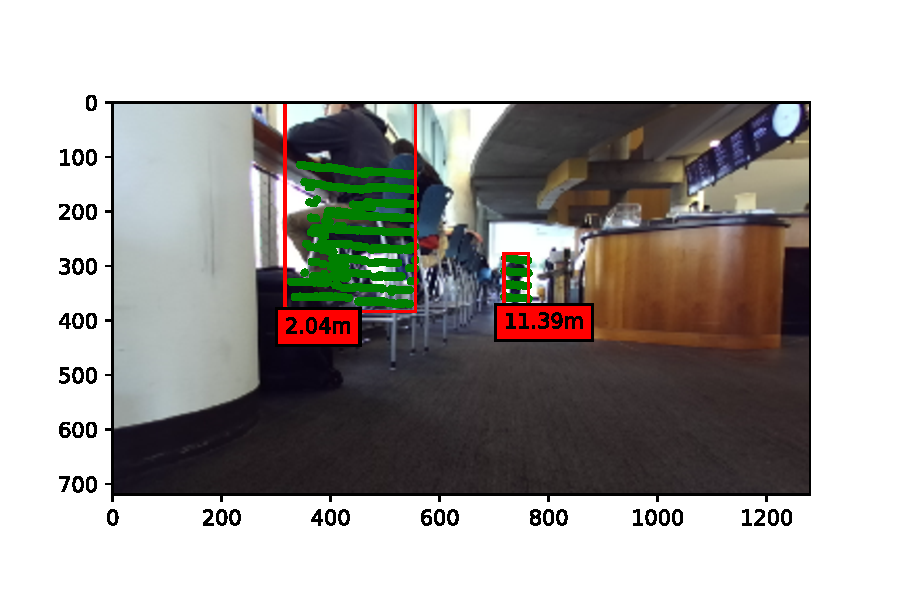
\includegraphics[height=5.0cm,width=0.7\columnwidth]{figs/visDet3D.pdf}
    % \end{subfigure}
    \caption{Multi-modal ground truth generation. The two red bounding boxes indicate people detected by Faster R-CNN. The green points are projected to the image from the LIDAR, with the relative distance between LIDAR and person shown as well.}\label{fig:gt}
\end{figure}

\section{Comparison with Existing Datasets}
In Table \ref{tab:data}, we compare our proposed dataset with existing datasets recorded from egocentric viewpoint in terms of (1) number of near-collision video sequences, (2) structure of scenes, and (3) setup used for recording. UAV crashing \cite{gandhi} dataset is created by crashing the drone 11,500 times into random objects. DroNet \cite{DroNet} has over 137 sequences of starting far way from an obstacle and stopping when the camera is very close to it. The two main reasons for collecting proposed dataset over existing datasets of UAV crashing and DroNet are: (1) applicability to assistive suitcase system \cite{BBeep}, and (2) focus on pedestrian motion. While the dataset provided by Ess et al \cite{Andreas} suited to our application, we find only $350$ near-collision instances making it infeasible to deploy CNNs.     




\clearpage

\chapter{Approach}
\label{chape:approach}
Our goal is to predict the time at which at least one person is going to come within a meter distance of the mobile setup using only a monocular image sequence of $N$ frames. The video is recorded at $10$ fps and thus a sequence of $N$ frames, including the current frame and past $(N-1)$ frames, correspond to the history of $\frac{N-1}{10}$ seconds. We first provide a formal definition of the task and then the details of network architecture for reproducibility.   

\section{Problem Formulation - Classification or Regression?}

Learning time to near-collision can be formulated as a multi-class classification into one of the 60 classes where $i^{th}$ class corresponds to time range between $(\frac{i-1}{10}, \frac{i}{10}]$ seconds. The disadvantage of training it as a classification task is that all the mispredictions are penalized equally. For example, let us consider two different mispredictions given the same ground truth of 0.5 seconds - one where the network categorized it into the class $(0.6, 0.7]$ and other when the network predicted $(5.5, 5.6]$. The multi-class cross-entropy loss on both of these will be equal while we want the latter to be penalized much more than the former. Thus, we formulate it as a regression problem and use the mean-squared error as the loss function. In this work, we formulated it as a regression problem as follows:
$$
%t = f(image_{1}, image_{2}, \hdots, image_{N}) \text{ where } t \in [0, 6]
t = f(I_{1}, I_{2}, \hdots, I_{N}) \text{ where } t \in [0,6]
$$

\section{Network Architecture}
%% Why I chose VGG-16?
%% ImageNet do not have a person class, thus the network was fine-tuned on PASCAL VOC dataset 
%% We propose a N-stream network where each stream takes in the $i^{th}$ image  
VGG-16 \cite{vgg} is a 16-layer convolutional neural network which won the localization task in ImageNet Challenge 2014. It used parameter efficient $3 \times 3$ convolutional kernels pushing the depth to 16 weight layers. It was shown that its representations generalize well to other datasets achieving state-of-the-art results. We propose a multi-stream VGG architecture as shown in Fig. \ref{fig:model} where each stream takes a $224 \times 224$ RGB frame as input to extract spatial features . These spatial features are then concatenated across all frames preserving the temporal order and then fed into a fully-connected layer to output time to collision. \\

% The inputs to the network are short N-frame clips corresponding to a temporal footprint of $\frac{N-1}{10}$ seconds. The concatenated features are fed into a 2 layer perceptron to give a single real-valued output. The network is trained using mean squared error as loss on the output. \\

\textbf{Feature Extraction from VGG-16} \\
We extracted the features of dimensions  7$\times$7$\times$512 from the last max pool layer of VGG-16. These features pass through an additional convolution layer to reduce the feature size to 7$\times$7$\times$16 and then flattened. These flattened features for each frame are concatenated into a vector and fed into the successive fully-connected layer of size 2048 which finally leads to a single neuron denoted as $t$ in Fig. \ref{fig:model}.  
%The network is trained using mean squared error as loss on the output.    \\
%% Which layer of VGG-16; I also added a conv layer from 512 channels to 16. 

In this network, the convolutional operators used spatial 2D kernels. A major question in current video architectures is whether these 2D kernels should be replaced by 3D spatio-temporal kernels \cite{i3d}. To answer this we also experimented with 3D spatio-temporal kernels and report the results in chapter \ref{chap:experimental_evaluation}. \\

\textbf{Training N-stream VGG} \\
We initialized the VGG-16 network using ImageNet-pretrained weights. As the ImageNet dataset does not have a person class, we fine-tuned the network weights on PASCAL VOC \cite{pascalVOC} dataset. Using these weights as initialization, we train a multi-stream architecture with shared weights. The network is trained using the following loss function.
$$
L_{MSE} = \frac{1}{2}||t_{true} - f(I_1, I_2, \hdots, I_N)||^{2}
$$
Here, $L$ is the mean squared loss between the predicted time, \emph{i.e.}, $f(I_1, I_2, \hdots, I_N)$ and ground truth time denoted as $t_{true}$. \\
The loss is optimized using mini-batch gradient descent of batch size 24 with the learning rate of $0.001$. The training data is further doubled by applying horizontal flip transformation.
%% Leaning rate, gradient descent, batch size

\clearpage

\chapter{Experimental Evaluation}
\label{chap:experimental_evaluation}
We now describe our evaluation procedure to decide the optimum temporal window as input on two different video network architectures. We further compare the performance with strong collision prediction baselines.


\section{Different temporal windows as input}
A single image can capture spatial information but no motion characteristics. Thus, we propose to use a sequence of image frames as history.  By feeding $N$ image frames, we consider a history of $\frac{N-1}{10}$ seconds. The temporal window of input frames was gradually increased from 2 frames (0.1 sec) to 9 frames (0.8 sec). To quantify the performance, we measure the mean absolute error (MAE) for the predictions on the test set and the standard deviation in error. From Table \ref{tab:hist}, it is empirically concluded to use a temporal window of 0.5 seconds, i.e, 6 frames for most accurate predictions. 

\begin{table}[ht]
\caption{Distribution of absolute error (mean $\pm$ std) on near-collision dataset using different number of input frames}\label{tab:hist}
\begin{tabular}{|P{3.75cm}|P{3.75cm}|P{3.75cm}|} \hline
Number of frames & Multi-stream VGG  & I3D  \\ \hline 
1 & 0.879 $\pm$ 0.762s & 0.961 $\pm$ 0.707s  \\ \hline
2 & 0.828 $\pm$  0.739s & 0.879 $\pm$ 0.665s \\ \hline 
3 & 0.826  $\pm$  0.647s & 0.914 $\pm$ 0.659s \\ \hline 
4  & 0.866 $\pm$  0.696s & \textbf{0.811 $\pm$ 0.642s}  \\ \hline
5 & 0.849 $\pm$ 0.734 & 0.849 $\pm$ 0.734s \\ \hline 
6  & \textbf{0.753 $\pm$ 0.687s} & 0.816 $\pm$ 0.663s   \\ \hline
7 & 0.757 $\pm$  0.722s & 0.848 $\pm$ 0.733s \\ \hline
8 & 0.913 $\pm$ 0.732s & 0.811 $\pm$ 0.647s \\ \hline 
9 & 0.817 $\pm$  0.738s & 0.855 $\pm$ 0.670s \\ \hline
\end{tabular}
\end{table}

\section{Experimental comparison of architectures}
We show a comparison of the performance of multi-stream VGG model and baselines including state-of-the-art methods in Table \ref{tab:baselines}. 

\begin{table}[ht]
\caption {Distribution of absolute error (mean $\pm$ std) on regression task compared with different baselines} \label{tab:baselines} 
\begin{tabular}{|P{6cm}|P{3cm}|P{2.25cm}|} \hline
Method  &  Mean (in s) & Std (in s)\\ \hline
Constant baseline ($\mathbb{E}[y_{true}]$) & 1.382 & 0.839\\ \hline 
Tracking + Linear Model \cite{BBeep} &  1.055  & 0.962 \\ \hline 
DroNet \cite{DroNet} & 1.099 &  0.842  \\ \hline 
Gandhi et al \cite{gandhi} & 0.884 & 0.818 \\ \hline
Single Image VGG-16 & 0.879  & 0.762 \\ \hline
I3D (4 frames) \cite{i3d} & 0.811  & 0.642  \\ \hline
\textbf{Multi-stream VGG (6 frames)} & \textbf{0.753}  & \textbf{0.687}  \\ \hline 
\end{tabular}
\end{table}

  \begin{figure}[ht]
      \centering
      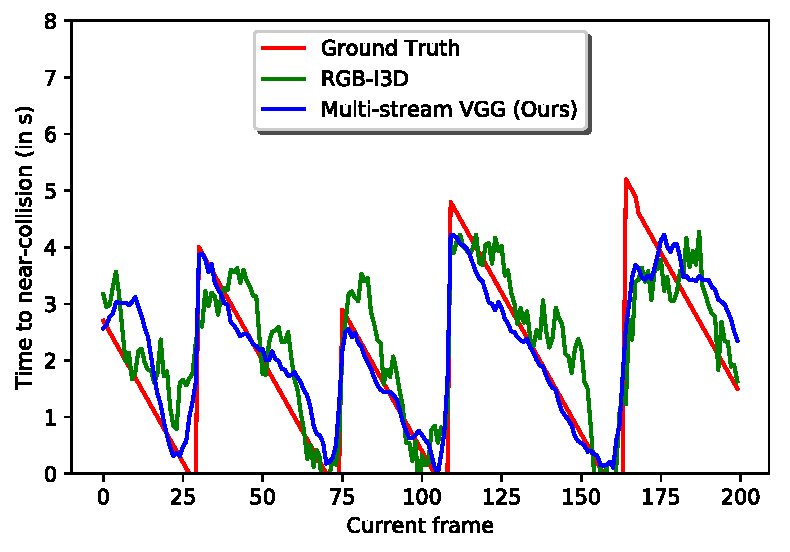
\includegraphics[height=7.5cm, width=\textwidth]{figs/400_new.pdf}
      \caption{Prediction of multi-stream VGG is smoother than I3D. The discontinuities here arise in the absence of pedestrians.}
      \label{fig:plot}
  \end{figure}
  
    \begin{figure*}[ht]
      \centering
      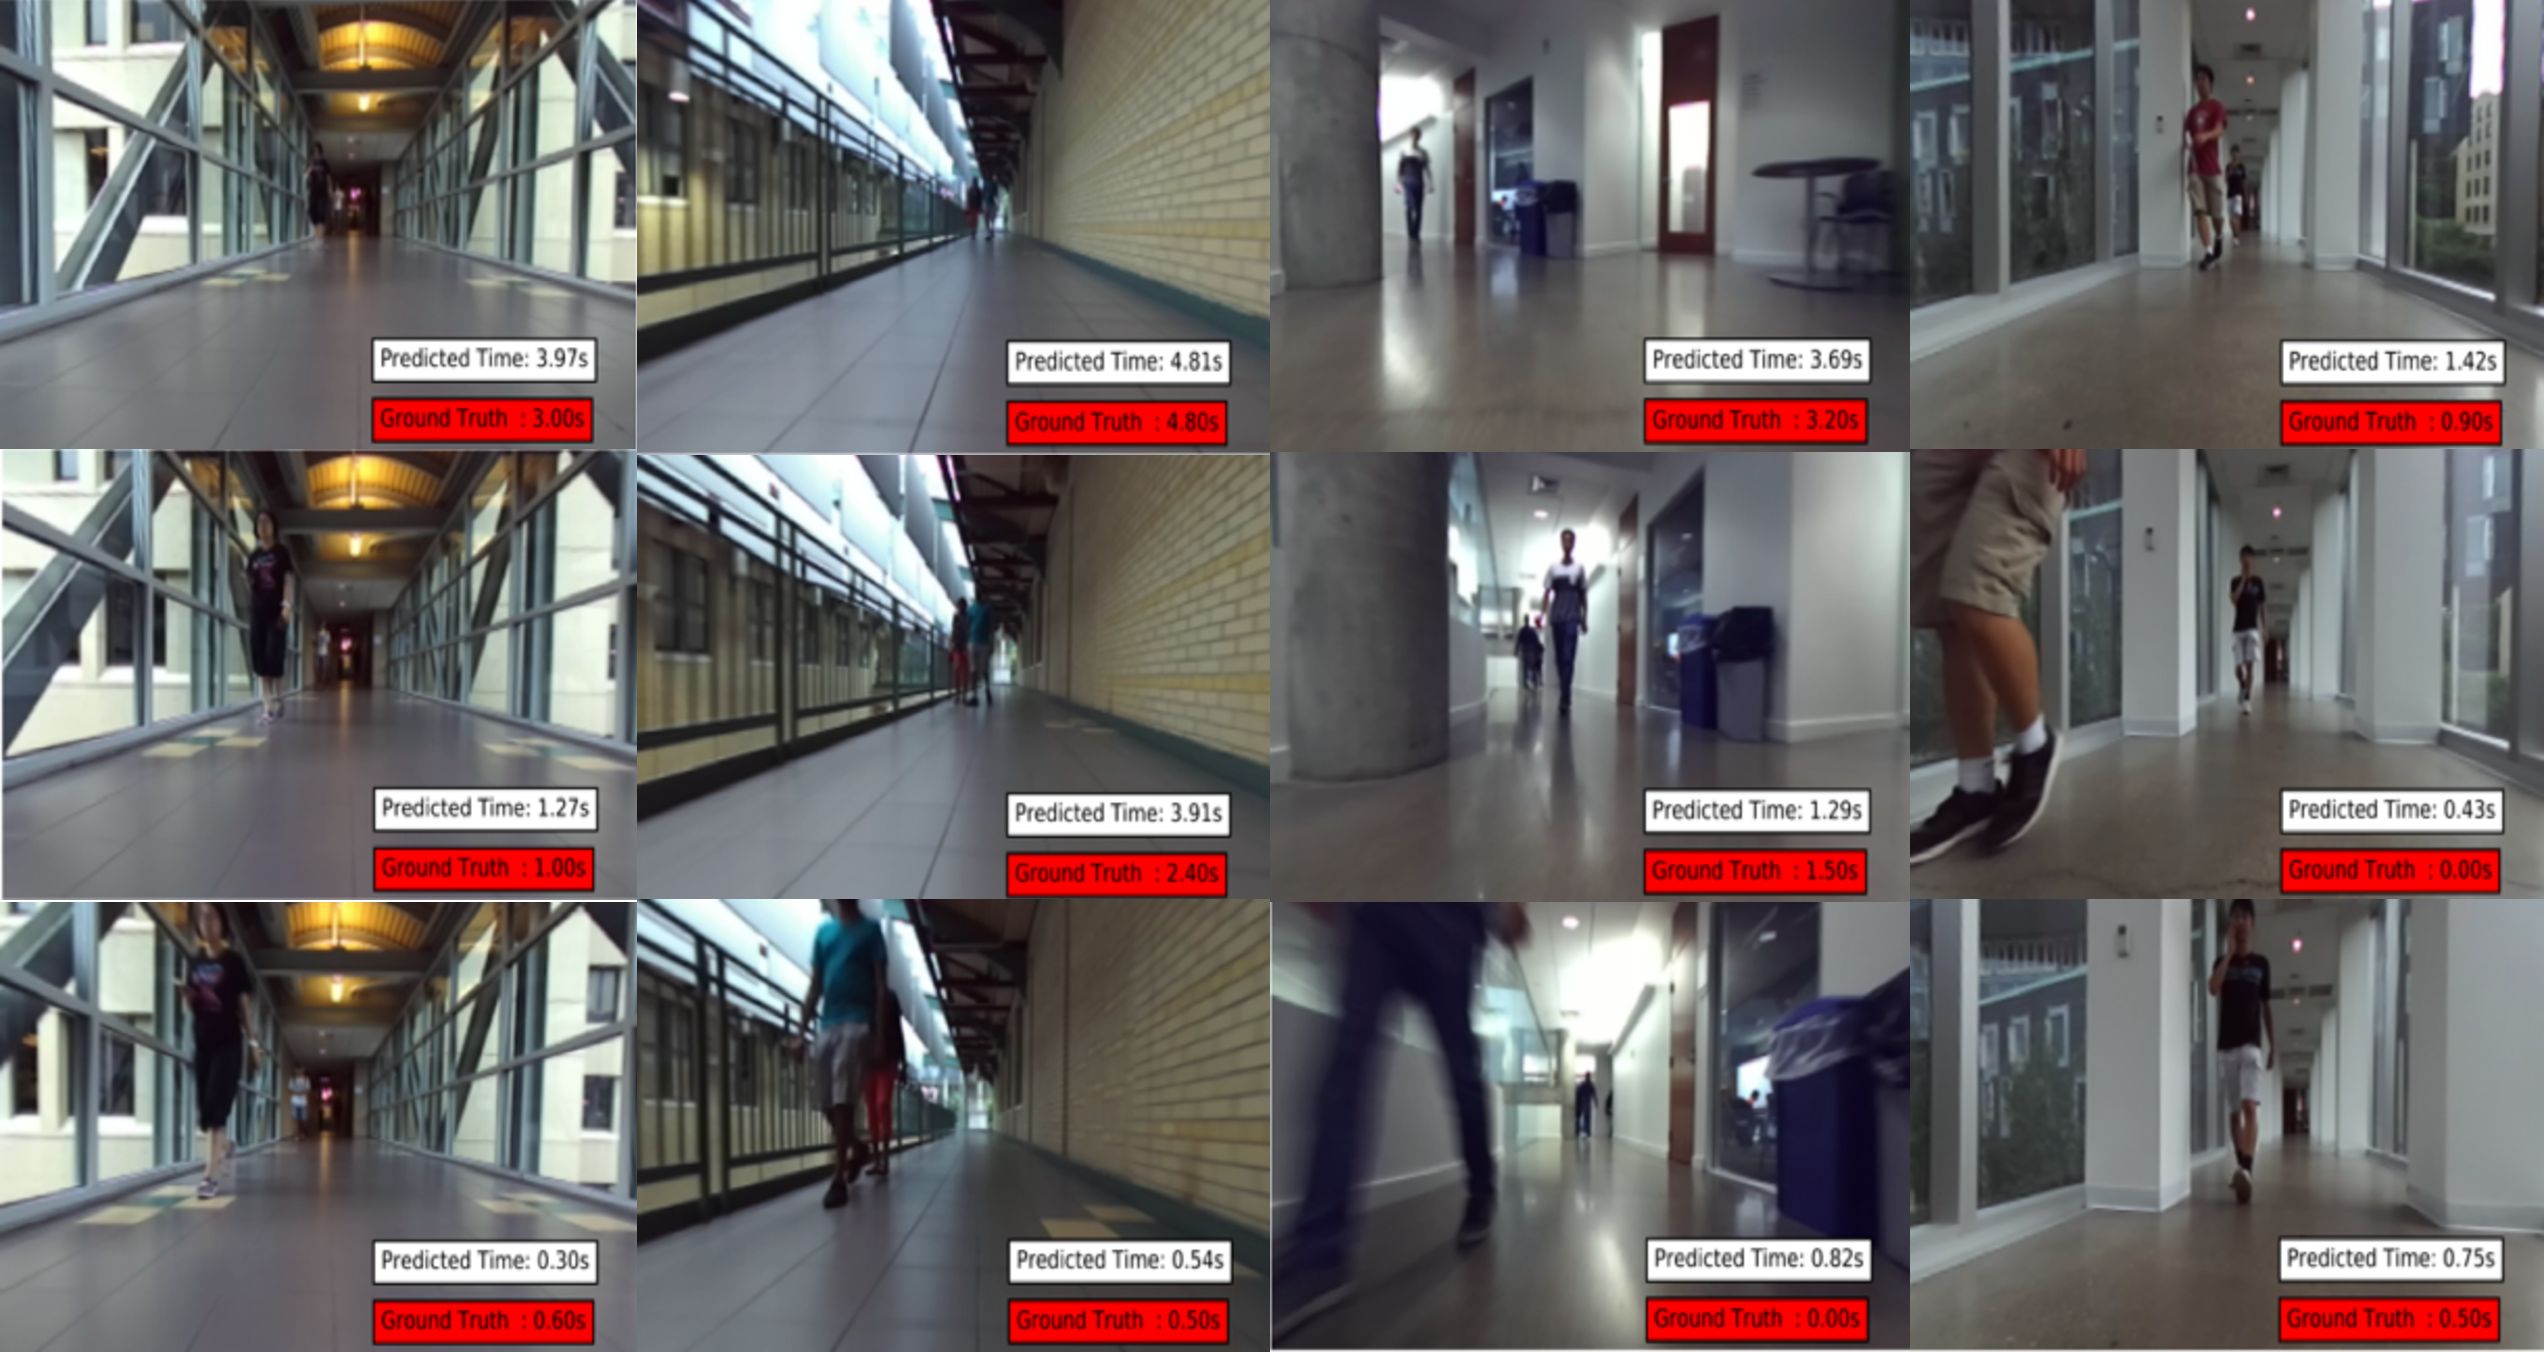
\includegraphics[height=10cm,width=\linewidth]{figs/qr2.pdf}
      \caption{Predictions on four different test videos}
      \label{fig:testVideos}
  \end{figure*}


\begin{enumerate}
    \item \textit{Constant Baseline:} On the training data of 12,620 samples, we compute the mean time to proximity denoted by $\mathbb{E}[y_{true}]$ as a weak baseline. For each test input, we predict $\mathbb{E}[y_{true}]$ which was found to be $2.23$ seconds. 
    
    \item \textit{Tracking followed by constant velocity model:} In dynamic environments, pedestrians are often tracked using a stereo camera or LIDAR. By saving few previous locations (0.5-2 seconds), a linear regression fit is used to predict the velocity vector of person \cite{BBeep}, \cite{SIPP}. This velocity vector is then linearly extrapolated to predict where the pedestrian will be over the next 6 seconds and the corresponding accuracy is reported in Table \ref{tab:baselines}. A major disadvantage in this method is the need for image-based tracking which is less reliable at low framerate of $10$ fps.     
    \item \textit{Deep learning for collision avoidance:} Collision avoidance using deep learning has been previously proposed in \cite{gandhi} and \cite{DroNet}. Gandhi et al \cite{gandhi} created a UAV crash dataset to train AlexNet for classifying the current image into one of these three categories of drone policy: go straight, turn left or turn right. For learning time to near-collision using their approach, we take a single image as input and use AlexNet architecture with ImageNet-pretrained weights as initialization. The only difference lies in the output layer which is a single neuron regression instead of a three-neuron classifier. Our multi-stream VGG outperformed current-frame AlexNet as reported in Table \ref{tab:baselines}.
    
ResNet-8 architecture used in DroNet \cite{DroNet} takes in the single image and after the last ReLU layer splits into two fully-connected streams outputting steering angle and collision probability respectively. To experiment with their learning approach, we used ResNet-8 architecture with only one output, i.e., time to near-collision. The performance is close to the constant velocity prediction model as reported in Table \ref{tab:baselines} and thus it can be seen that it is unable to leverage real-world data. One of the reasons for its low performance could be the unavailability of ImageNet-pretrained weights for ResNet-8 architecture and thus it has to be trained from scratch on our proximity dataset which is much smaller than the Udacity's car-driving dataset of 70,000 images used for training steering angle stream in DroNet.   
    
    %% should elaborate in related work 
    %% Here only the network architecture and why is it chosen as a baseline 
    \item \textit{I3D for action classification in videos:} Two-Stream Inflated 3D ConvNet (I3D) \cite{i3d} is a strong baseline to learn a task from videos. All the $ N \times N$ filters and pooling kernels in ImageNet-pretrained Inception-V1 network \cite{inceptionv1} are inflated with an additional temporal dimension to become $N \times N \times N$. I3D has two streams - one trained on RGB inputs and other on optical flow inputs. To avoid adding the latency of optical flow computation for real-time collision forecasting, we only used the RGB stream of I3D. We fine-tuned the I3D architecture which was pre-trained on Kinetics Human Action Video dataset \cite{i3d} on our near-collision dataset by sending $N$ RGB frames as input where $N = \{1,2, \hdots, 8,9\}$ as reported in Table \ref{tab:hist}. The outermost layer is modified from 400-neuron classifier to 1-neuron regressor. Since our $N$-frame input is smaller than the original implementation on 64-frame input, we decreased the temporal stride of last max-pool layer from 2 to 1. While 6 input frames were found to be the best for proposed multi-stream VGG network, we experimented again with the optimal history on I3D. The performance of I3D with varying number of input frames is reported in Table \ref{tab:hist}.  For $N = 4, 6, 8$, I3D is found to give the best results among 1-9 frames though our multi-stream VGG prediction for $N = 6$ outperformed the I3D prediction in best case. 
\end{enumerate}
\section{Qualitative Evaluation}
% After seeing quantitative results as reported in Table \ref{tab:baselines}, the mean absolute error between proposed approach and the closest baseline I3D differs by a small number of 0.05 seconds. Does it mean that the proposed method offers only a slight improvement over existing approaches which might be negligible during real-time execution? To answer this we plotted the predictions made by proposed network and most competitive baseline I3D to compare with the ground truth. 
From the plots shown in Fig. \ref{fig:plot} we can observe that the predictions given by multi-stream VGG on 6 frames give smoother output as compared to undesired fluctuations in I3D output. We also qualitatively show in Fig. \ref{fig:testVideos} the comparison of time to near-collision predicted by our method vs the ground truth. 
%This motivates the introduction of another evaluation metric - smoothness factor. 


\clearpage

\chapter{Conclusion}
\label{chap:discussion}
We return to the question posed in introduction, 'Is it possible to predict the time to near-collision from a single camera?'. The answer is that the proposed model is able to leverage spatio-temporal cues for predicting the time to collision within $0.75 \pm 0.68$ seconds on the test videos. Also, we observed that the multi-stream network of shared weights performed the task of collision forecasting better than I3D on the proposed dataset. 
%One of the major boosts to multi-stream VGG is the reuse of VGG-16 network pretrained on PASCAL VOC classification dataset which contains cimages of person class whereas I3D is pretrained Kinetics Human Action Video. 

With regard to temporal window of input history, it is evident that using a sequence of images has a considerable benefit over prediction from single frame only. Though the history of 0.5 seconds performed best, we do not observe a piecewise monotonic relation between input frames and error in prediction. This observation aligns with the performance of constant velocity model where accuracy in prediction does not necessarily increase or decrease with the temporal footprint of past trajectory. 

We understand that the proposed model might not generalize well when there are large changes in camera's height or structure of the scenes in comparison to provided dataset. In the scenarios where assistive robot operates in a constrained domain like museums and airports, the proposed approach will be suitable for predicting time to collision requiring only a low-cost monocular camera.

\clearpage

\chapter{Future Work}
\label{chap:future_work}
One of the scenarios where the proposed approach fails is when a person is moving in the same direction as user. The pedestrian detector detects the person and so the image is passed through the proposed multi-stream network. The network outputs an inaccurate estimate of time-to-collision as shown in Figure \ref{fig:misprediction}.

\begin{figure}[ht]
    \centering
        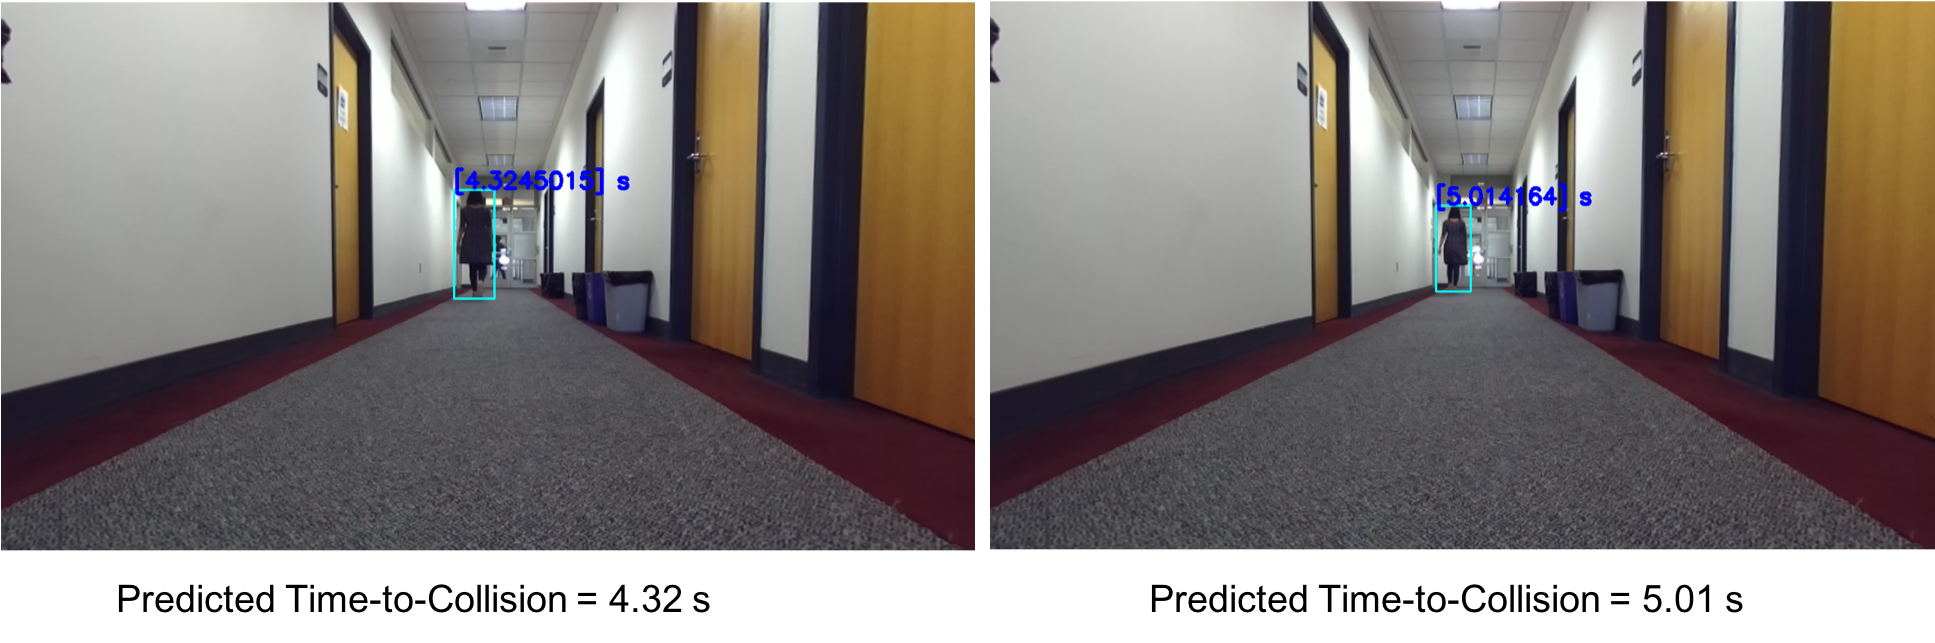
\includegraphics[height=5.0cm,width=\textwidth]{figs/mispredictions.png}
    \caption{Inaccurate estimate of time-to-collision when a person is moving away from the assistive suitcase}\label{fig:misprediction}
\end{figure}

Instead of passing the image first through the pedestrian detector, if we can instead pass it through a binary classifier trained to classify if there is going to be a collision within the chosen time bound (here, 6 seconds) or not. If positive, we can then pass it through the regressor network as proposed in this work to estimate the exact time-to-collision. OpenPose \cite{OpenPose}, a realtime approach to detect the 2D pose of multiple people in an image including foot, torso, arms and face keypoints can be leveraged to replace the object detection backbone, i.e, VGG-16 to enhance the prediction performance. \\

The prediction time bound in this work is chosen to be 6 seconds arbitrarily. Depending on the application or the planner requirements, the time bound could be chosen accordingly. For a higher time bound, it would be challenging to learn the task within an acceptable error limit. The Table \ref{tab:different_horizons} reports how the error varies with prediction time horizon.
\begin{table}[h]
\caption {Mean Absolute Error in Predicted Time varying with the Prediction Time Horizon} \label{tab:different_horizons} 
\begin{tabular}{|P{0.45\textwidth}|P{0.45\textwidth}|} \hline
Prediction Time Horizon (in seconds)  &  Mean Absolute Error (in seconds) \\ \hline
5 &  0.565 \\ \hline 
6 &  0.753 \\ \hline %% From slides
7 & 0.903 \\ \hline
\end{tabular}
\end{table}



\clearpage 

%Include references using bst and bib files.
\bibliographystyle{finitplain} 
{\small \bibliography{local}}


\end{document}
